%!TEX root =  main.tex
\section{Varying the Epsilon Allocation}
Since the $F_1$-statistic outperforms the other $F_q$-statistics, we will proceed by discussing only the $F_1$-statistic. In Algorith~\ref{alg:F1}, we divide the epsilon budget equally between the numerator and denominator of the statistics by allocating $\epsilon/2$ to each of \sa and \se. This is a perfectly reasonable starting point. We wondered if allocating more of the epsilon budget to the \sa would improve the power of the statistic, since we use $\sa/(\dbsize - \k)$ as our standard deviation estimate\ab{I thought we used SE/N?}. This modifies our algorithm slightly; rather than allocating \eps/2 to each of \sa and \se, we will allocate a portion $\epsfrac \cdot \eps$ to the \sa  computation, and $(1-\epsfrac)\cdot \eps$ to the \se computation, where $\epsfrac \in [0,1]$.  In other words, \epsfrac is the proportion of our epsilon budget that we will allocate to the \sa computation. This proportion could potentially be user-defined, but we found a particular value for \epsfrac to be superior, so it will be a constant. We used the same method for calculating the $p$-value for a statistic as the regular $F_1$ (Algorithm~\ref{alg:pval}).

Our updated algorithm is as follows: \ms{Not sure if it's clear enough to just describe or if we want to have the full algorithm. I put it in here so we can decide later}
\begin{algorithm}
    \caption{Differentially private ANOVA with Absolute Values and varying Epsilon Allocation \label{alg:F1epsfrac}}
    \begin{algorithmic}
        \STATE \textbf{Input:} Database $\x$, $\eps$ value, epsilon allocation $\epsfrac \in (0,1)$
        \STATE Compute $\widehat{\sa} = \sa(x) + Z_1$ where $Z_1\sim\text{Lap}\left(\frac{4}{\eps\cdot\epsfrac}\right)$
        \STATE Compute $\widehat{\se} = \se(x) + Z_2$ where $Z_2\sim\text{Lap}\left(\frac{3}{\eps\cdot(1-\epsfrac)}\right)$
        \STATE Compute $\widehat{F_1} = \frac{\widehat{\sa}/(k-1)}{\widehat{\se}/(n-k)}$
        \STATE \textbf{Output:} $\widehat{F_1}, \widehat{\sa}, \widehat{\se}$
    \end{algorithmic}
\end{algorithm}

\begin{theorem}
Algorithm~\ref{alg:F1epsfrac} is \eps -differentially private.
\end{theorem}
\begin{proof}
As before, we use the Laplace Mechanism (Definition~\ref{thm:lapmechanism}) to compute the \sa and \se with privacy $\eps\cdot\epsfrac$ and $\eps\cdot(1-\epsfrac)$, respectively. Since the number of groups \k and total database size \dbsize are public information, computing $\widehat{F_1}$ is post-processing (Theorem~\ref{thm:postprocessing}) and does not affect the privacy of Algorithm~\ref{alg:F1epsfrac} . Thus, by the composition theorem (Theorem~\ref{thm:composition}), Algorithm~\ref{alg:F1epsfrac} is $\eps\cdot\epsfrac + \eps\cdot(1-\epsfrac) = \eps$-differentially private.
\end{proof}

\subsection{Optimal \epsfrac for $F_{1}$}
We constructed power plots comparing database size to power for different \epsfrac values. We began by exploring the full range from $0.1$ to $0.9$ by $0.1$-increments to get a sense of the differences in power between these variants of the $F_1$-statistic. After that initial pass, we tuned in to the value with higher precision. We tried this for multiple effect sizes and surprisingly found that $\epsfrac = 0.5$ was not optimal for the effect sizes that we tried.\ms{we should be more specific about the effect sizes once we have the plots, etc.}  We found that across many effect sizes, $\epsfrac = 0.7$ was the most powerful. We hypothesize that this difference comes from  either the difference in sensitivities of \sa and \se, or that having an accurate numerator contributes more to the overall accuracy of the statistic (?). \ms{Someone find an intelligent justification for this} \ar{Any justification will need to be backed up with a result -- think about how you could test this hypothesis.  If it remains speculative, it should go in the Discussion/Conclusion section, not in Results.}  Since we are not able to compute the optimal \epsfrac analytically, we resort to simulation across many effect sizes and database sizes to find the best \epsfrac.
\begin{figure}
\centering
\includegraphics[width=\linewidth]{F1-epsfrac.png}
%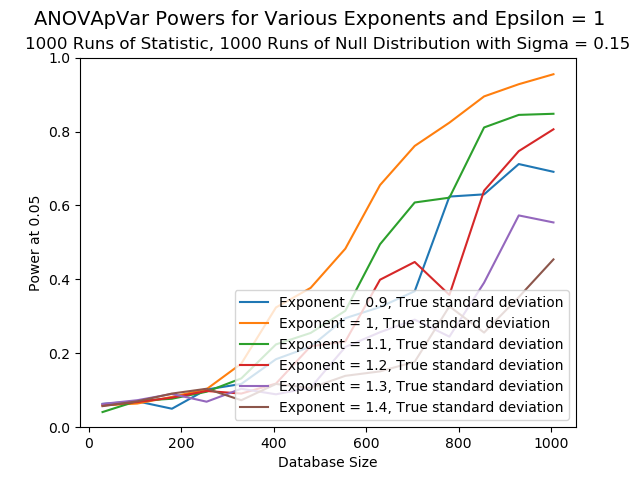
\includegraphics[width=0.8\textwidth,natwidth=610,natheight=642]{Placeholder_manyExponents.png}
\caption{Power is experimentally maximized when $\rho = .7$.}
\end{figure}
\ms{Insert some kind of graph or table illustrating the point and  illustrating the power gained from using the new epsfrac} \ar{Yep, good idea.}
